\appendix
\section{Deferred proofs}
\label{app:deferred-proofs}



\subsection{Equal-reliability optimum}

\begin{lemma}
\label{lem:equalrel}
For $p$ honest and $q$ inverted sources, all with reliability $r > 1/2$
and full stability ($\rho = 1$), the Bayes accuracy is
\[
A_{\mathrm{Bayes}} = P\!\left(\mathrm{Bin}(p+q, r) > \tfrac{p+q}{2}\right)
+ \tfrac{1}{2}P\!\left(\mathrm{Bin}(p+q, r) = \tfrac{p+q}{2}\right),
\]
while the best unsigned (nonnegative-weight) rule attains only
\[
A_{\mathrm{unsigned}} = P\!\left(\mathrm{Bin}(p, r) > \tfrac{p}{2}\right)
+ \tfrac{1}{2}P\!\left(\mathrm{Bin}(p, r) = \tfrac{p}{2}\right),
\]
i.e.\ it optimally discards the inverted sources ($w_j = 0$).
\end{lemma}



Numerically, for $p=2$, $q=1$, $r=0.8$:
$A_{\mathrm{Bayes}} = 0.896$ versus $A_{\mathrm{unsigned}} = 0.80$; for
$p=3$, $q=2$, $r=0.8$: $0.942$ versus $0.896$. So nonnegative weighting
does not merely underperform. Its optimal strategy is to throw away
informative sources entirely. Thus, under this regime, the optimal
unsigned rule discards the inverted sources rather than exploiting their
information.

\begin{proof}
Work in $\{\pm 1\}$ encoding. With $\rho = 1$, honest sources emit
$X_s = Z_s$ and inverted sources emit $X_{p+j} = -Z_{p+j}$, where the
readings $Z_i$ are conditionally independent given $Y$ with
$P(Z_i = Y) = r$. An unsigned rule computes
$\mathrm{sign}\bigl(\sum_{s=1}^p w_s Z_s + \sum_{j=1}^q v_j Z'_{p+j}\bigr)$
with $w_s, v_j \geq 0$, where $Z'_{p+j} = -Z_{p+j}$ satisfies
$P(Z'_{p+j} = Y) = 1 - r < \tfrac{1}{2}$: each inverted message is
\emph{negatively} informative about $Y$.

\textit{Step 1: negative information is worse than noise.}
Fix an inverted source $j$ and write the score as $v_j Z'_j + T$, where
$T$ collects all other terms. Conditional on $(T, Y) = (t_0, y)$,
\[
P(\text{correct} \mid t_0, y)
= (1-r)\,\mathbb{1}[\mathrm{sign}(v_j y + t_0) = y]
+ r\,\mathbb{1}[\mathrm{sign}(-v_j y + t_0) = y],
\]
using $P(Z'_j = y \mid Y = y) = 1 - r$ and conditional independence of
$Z'_j$ from $(T, Y)$ given $Y$. Replace $Z'_j$ by a fair coin $C_j$
independent of everything: the conditional accuracy becomes
$\tfrac{1}{2}\mathbb{1}[\mathrm{sign}(v_j y + t_0) = y]
+ \tfrac{1}{2}\mathbb{1}[\mathrm{sign}(-v_j y + t_0) = y]$.
The difference (coin minus $Z'_j$) is
\[
(r-\tfrac{1}{2})\Bigl(\mathbb{1}[t_0 y > -v_j]
- \mathbb{1}[t_0 y > v_j]\Bigr) \geq 0,
\]
since $r > \tfrac{1}{2}$ and $-v_j \leq v_j$ (ties broken symmetrically
preserve monotonicity). Hence replacing each inverted source's message
by pure noise \emph{weakly improves} every unsigned rule. Iterating over
$j = 1, \dots, q$,
\[
A(w, v) \leq
P\!\left(\mathrm{sign}\!\left(\sum_{s=1}^p w_s Z_s
+ \sum_{j=1}^q v_j C_j\right) = Y\right),
\]
with $C_j$ i.i.d.\ fair coins independent of $(Z, Y)$.

\textit{Step 2: noise cannot beat the honest-only Bayes rule.}
Write $S = \sum_{s=1}^p w_s Z_s$ and $N = \sum_{j=1}^q v_j C_j$.
Since $N$ is independent of $(S, Y)$ and symmetric,
\[
P(\mathrm{sign}(S + N) = Y)
= \mathbb{E}_N\bigl[P(\mathrm{sign}(S + n) = Y)\bigr].
\]
For each fixed $n$, $\mathrm{sign}(S + n)$ is a deterministic function
of the honest readings alone, so its accuracy is bounded by the
honest-only Bayes accuracy: the majority vote over decoded readings,
$P(\mathrm{Bin}(p,r) > p/2) + \tfrac{1}{2}P(\mathrm{Bin}(p,r) = p/2)$.
Thus $A(w, v) \leq A_{\mathrm{unsigned}}$ for all $w, v \geq 0$.

\textit{Step 3: achievability.} Setting $v_j = 0$ and equal $w_s > 0$
gives exactly the honest-only majority vote, attaining the bound. The
Bayes formula follows identically with all $p+q$ decoded readings.
\end{proof}

\subsection{Proof of Theorem~\ref{thm:scalar}}
\begin{proof}
(a) Consider source $j$ in isolation. Because $f_{c_j}$ is an involution in
its first argument, the observed raw message $M_j$ decodes to the reading
$d^{(t)} = f_{c_j}(M_j, a^{(t)})$ (centered: $X_j = 2M_j - 1$).
Context-dependence gives
$d^{(1)} \neq d^{(2)}$ for suitable $M_j$ (e.g.\ the XOR convention with
$M_j = v_j \oplus a^{(1)}$). With stability $\rho = 1$, the per-source
log-odds are $+\lambda_j$ when the decoded reading is $1$ and
$-\lambda_j$ when it is $0$, so the Bayes decision is $+1$ on $x^{(1)}$
and $-1$ on $x^{(2)}$ (or vice versa) while the message vector $X$ is
identical.

(b) Any context-independent rule is a function $f(X)$ of the message
vector alone, so it assigns identical predictions to $x^{(1)}$ and
$x^{(2)}$, contradicting (a).
\end{proof}

\subsection{Proof of Theorem~\ref{thm:consistency}}
\begin{proof}
Support triples $(M_i, a_i, Y_i)$ are i.i.d.\ across $i$. For any grid
point $\theta \notin [\theta^*]$, the mean log-likelihood ratio
\[
\frac{1}{K}\sum_{i=1}^K
\log\frac{P(M_i, a_i, Y_i \mid \theta^*)}{P(M_i, a_i, Y_i \mid \theta)}
\;\xrightarrow{a.s.}\;
D_{\mathrm{KL}}(P_{\theta^*} \,\|\, P_{\theta}) > 0
\]
by the strong law of large numbers, with strict positivity from the
definition of the equivalence class. The grid is finite, hence so is the
set of equivalence classes, and the minimum KL divergence to any class
other than $[\theta^*]$ is a positive constant $\delta > 0$. The posterior
odds of each foreign class against $[\theta^*]$ therefore decay as
$\exp(-K(\delta + o(1)))$, uniformly over the finitely many classes, so
$P([\theta^*] \mid \mathcal{D}_s) \to 1$ a.s.

For the predictive, write the log-odds at query $(M_q, a_q)$ as
$\log(N_K / D_K)$ with $N_K = \sum_\theta w_\theta\, p_1(\theta)$,
$D_K = \sum_\theta w_\theta\, p_0(\theta)$,
$w_\theta = P(\theta \mid \mathcal{D}_s)$, and
$p_y(\theta) = P(M_q \mid Y = y, a_q, \theta)$.
The query likelihood is the same conditional that appears in the
support-triple distribution, so $p_y(\theta) = p_y(\theta^*)$ for every
$\theta \in [\theta^*]$, for $P_A$-almost every query context $a_q$.
Hence $N_K = p_1(\theta^*) P([\theta^*] \mid \mathcal{D}_s) + R_K$ with
$|R_K| \le \max_\theta p_1(\theta)\,(1 - P([\theta^*] \mid \mathcal{D}_s))
\to 0$ a.s., and likewise for $D_K$. On the grid,
$p_y(\theta) \in [0.05, 0.95]$, so the logarithm is continuous at the
limit point and the predictive log-odds converge a.s.\ to
$\log(p_1(\theta^*)/p_0(\theta^*))$: the oracle's log-odds.
\end{proof}

\section{Deferred experimental details}
\label{app:deferred-exp}

\begin{table}[h]
\centering
\caption{The eight involutive conventions in the benchmark.}
\label{tab:conventions}
\begin{tabular}{clcc}
\toprule
ID & Convention & Involutive & Context-dependent \\
\midrule
0 & identity & yes & no \\
1 & NOT & yes & no \\
2 & XOR with $a_1$ & yes & yes \\
3 & XOR with $a_2$ & yes & yes \\
4 & XOR with $(a_1 \land a_2)$ & yes & yes \\
5 & XOR with $(a_1 \lor a_2)$ & yes & yes \\
6 & XOR with $(a_1 \oplus a_2)$ & yes & yes \\
7 & XOR with $\lnot(a_1 \land a_2)$ & yes & yes \\
\bottomrule
\end{tabular}
\end{table}

\subsection{Posterior diagnostic}

To check that the Bayesian inference actually identifies conventions rather
than stumbling into good predictions by accident, we measure top-1 accuracy
on the true convention ($0.828 \pm 0.040$) and posterior mass concentration
($0.722 \pm 0.032$ of sources put mass above $0.50$ on the true convention)
across 200 random sources with $K=20$. Decision accuracy is $0.831$ when the
top-1 convention is correct but still $0.686$ when it is wrong: the
posterior-predictive averages over convention uncertainty rather than
committing to a single convention, so decisions often survive
misidentification. Full details are in Appendix~\ref{app:deferred-exp}.

\subsubsection{Detailed diagnostic}

To check that the Bayesian inference actually identifies conventions
rather than stumbling into good predictions by accident, we measure top-1
accuracy on the true convention and posterior mass concentration across
200 random sources with $K=20$ (mean $\pm$ std over 10 seeds):

\begin{itemize}
\item Top-1 accuracy on the true convention: $0.828 \pm 0.040$.
\item Fraction of sources with posterior mass exceeding $0.50$ on the true convention: $0.722 \pm 0.032$.
\end{itemize}

These are diagnostics, not bounds. A diffuse posterior can still predict
well if its errors cancel, and a concentrated posterior can predict badly
if $r$ or $\rho$ are misestimated. What the numbers say is modest and
reassuring: the posterior usually finds the right convention, and the
predictive accuracy in \S6.1 and \S6.5 is consistent with that.

A natural follow-up is whether decisions survive convention
misidentification. Conditioning on recovery across the same 200 sources
per seed: decision accuracy is $0.831$ when the top-1 convention is
correct, but still $0.686$ when it is wrong, well above chance. The
posterior-predictive averages over the convention uncertainty rather than
committing to a single (possibly wrong) convention, so the aggregator
often gets the decision right even when it cannot name the code. Decision
accuracy, not convention-identification accuracy, is what matters, and the
Bayesian rule maintains decision accuracy on the former well above chance
even when the latter fails.

\begin{figure}[h]
\centering
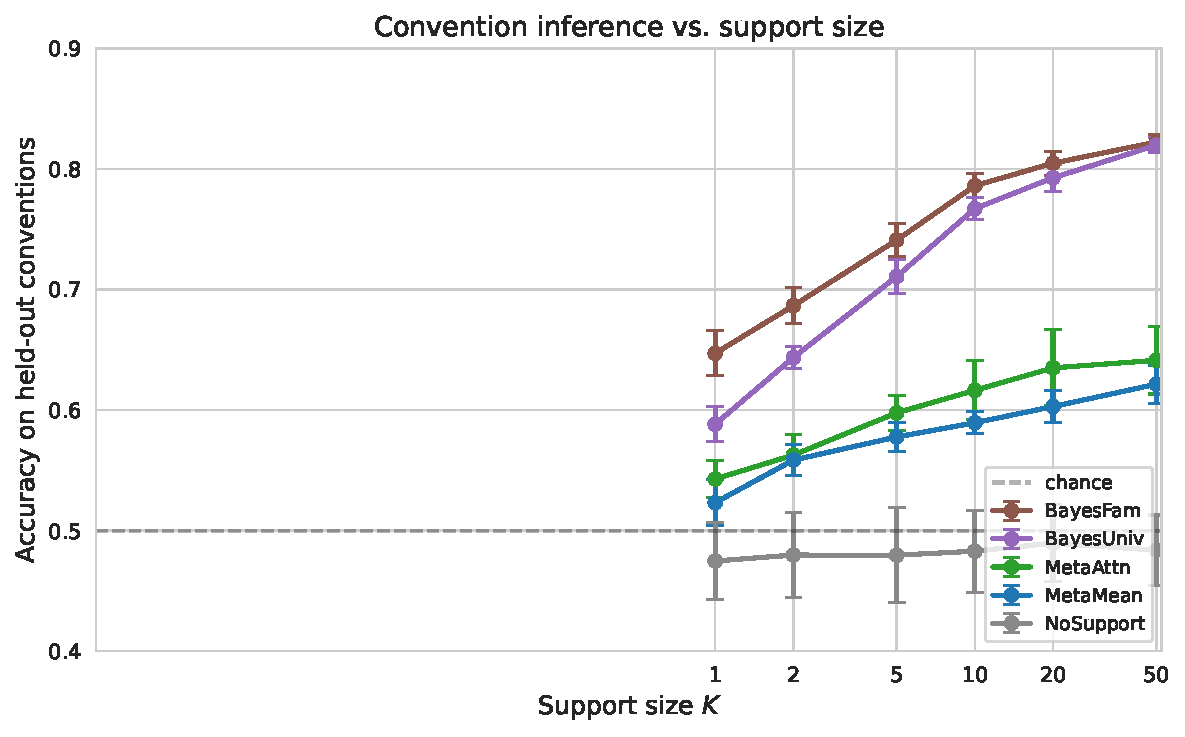
\includegraphics[width=0.85\columnwidth]{../figures/fig3_ksweep.pdf}
\caption{Accuracy on held-out conventions vs.\ support size $K$. Error bars show $\pm 1$ std over 10 seeds. Both Bayesian variants converge toward the per-query information ceiling ($\approx 0.82$); neural calibrators plateau near $0.64$.}
\label{fig:ksweep}
\end{figure}

\begin{figure}[h]
\centering
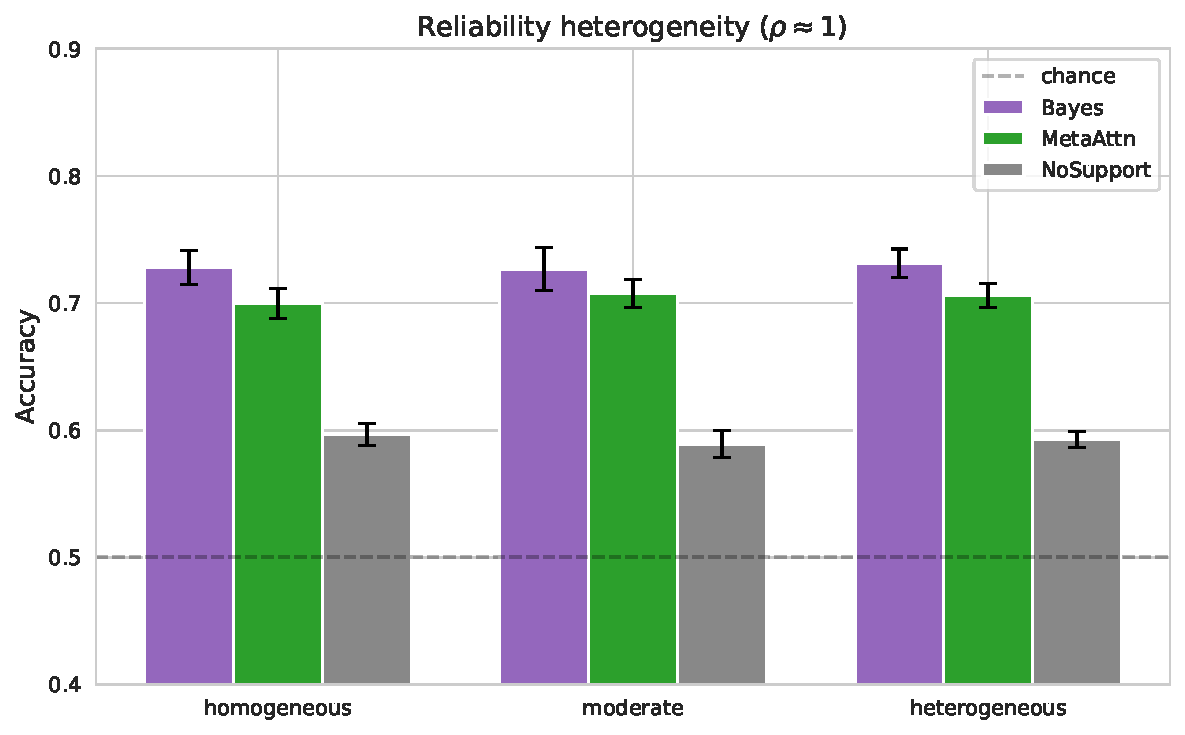
\includegraphics[width=0.85\columnwidth]{../figures/fig4_reliability.pdf}
\caption{Robustness to reliability heterogeneity ($\rho \approx 1$, mean-matched $\mathbb{E}[r]=0.80$). Error bars show $\pm 1$ std over 10 seeds. Accuracy tracks the mean reliability across spreads; heterogeneity per se does not degrade the Bayesian aggregator.}
\label{fig:reliability}
\end{figure}

\subsection{Robustness checks}
\label{sec:robustness}

Tables report mean $\pm$ std over ten seeds. 95\% confidence intervals
($t_{0.975,9} = 2.262$) confirm every headline gap: the $\rho$-sweep
monotonicity, the ablation ordering, the $+38.2$ point consensus margin and
$4.0$ point oracle gap at $N=12$, and the $7$ point misspecification drop.
Grid-resolution sweeps (96/432/1496 cells) move every headline number by at
most $0.004$, and a likelihood-temperature sweep preserves all orderings
except at the pathological $T=5.0$. Details are in
Appendix~\ref{app:robustness}.

\subsubsection{Detailed robustness results}
\label{app:robustness}

{\sloppy
Tables report mean $\pm$ std over ten seeds; here we add 95\% confidence
intervals ($t_{0.975,9} = 2.262$) and two sensitivity sweeps of the
Bayesian aggregator, implemented in torch-free NumPy drivers
(\texttt{code/ci\_check.py}, \texttt{code/sens\_bayes.py}) that reproduce
the paper's Bayes columns bit-identically on the default grid. Every
headline gap survives: in the $\rho$ sweep Bayes rises monotonically
($0.625 \pm 0.008$ to $0.755 \pm 0.009$, adjacent intervals
non-overlapping) and sits strictly above every baseline at $\rho=1$; in
the ablation Bayes ($0.758 \pm 0.011$) is strictly below the oracle
($0.825 \pm 0.006$) while the privileged \textsc{MetaAttn+Dec}
($0.822 \pm 0.006$) is within noise of it; at $N=12$ the $+38.2$ point
margin over naive averaging ($0.955 \pm 0.014$ vs.\ $0.573 \pm 0.044$) and
the $4.0$ point oracle gap both hold; the misspecification drop
($0.756 \pm 0.009$ to $0.685 \pm 0.008$) is real. The one comparison that
does \emph{not} survive is \textsc{ContextConditioned} vs.\
\textsc{MetaAttn} ($0.730 \pm 0.010$ vs.\ $0.722 \pm 0.009$): overlapping
intervals, a point-estimate ordering only, as reported in \S6.3. Grid
resolution is not a driver: coarsening the grid $4.5\times$ (96 cells) or
refining it $3.5\times$ (1496 cells) moves every headline number by at
most $0.004$. A likelihood-temperature sweep ($T \in \{0.5, 2.0\}$,
flattening or sharpening the posterior toward or away from the uniform
prior) preserves all orderings; only at the pathological $T = 5.0$ do
magnitudes attenuate, and even there Bayes stays above the scalar
baselines. The quantitative claims are calibrated to the stated
uniform-prior model, and they are not prior-fragile.
\par}